\documentclass[twoside]{book}

% Packages required by doxygen
\usepackage{fixltx2e}
\usepackage{calc}
\usepackage{doxygen}
\usepackage[export]{adjustbox} % also loads graphicx
\usepackage{graphicx}
\usepackage[utf8]{inputenc}
\usepackage{makeidx}
\usepackage{multicol}
\usepackage{multirow}
\PassOptionsToPackage{warn}{textcomp}
\usepackage{textcomp}
\usepackage[nointegrals]{wasysym}
\usepackage[table]{xcolor}

% Font selection
\usepackage[T1]{fontenc}
\usepackage[scaled=.90]{helvet}
\usepackage{courier}
\usepackage{amssymb}
\usepackage{sectsty}
\renewcommand{\familydefault}{\sfdefault}
\allsectionsfont{%
  \fontseries{bc}\selectfont%
  \color{darkgray}%
}
\renewcommand{\DoxyLabelFont}{%
  \fontseries{bc}\selectfont%
  \color{darkgray}%
}
\newcommand{\+}{\discretionary{\mbox{\scriptsize$\hookleftarrow$}}{}{}}

% Page & text layout
\usepackage{geometry}
\geometry{%
  a4paper,%
  top=2.5cm,%
  bottom=2.5cm,%
  left=2.5cm,%
  right=2.5cm%
}
\tolerance=750
\hfuzz=15pt
\hbadness=750
\setlength{\emergencystretch}{15pt}
\setlength{\parindent}{0cm}
\setlength{\parskip}{3ex plus 2ex minus 2ex}
\makeatletter
\renewcommand{\paragraph}{%
  \@startsection{paragraph}{4}{0ex}{-1.0ex}{1.0ex}{%
    \normalfont\normalsize\bfseries\SS@parafont%
  }%
}
\renewcommand{\subparagraph}{%
  \@startsection{subparagraph}{5}{0ex}{-1.0ex}{1.0ex}{%
    \normalfont\normalsize\bfseries\SS@subparafont%
  }%
}
\makeatother

% Headers & footers
\usepackage{fancyhdr}
\pagestyle{fancyplain}
\fancyhead[LE]{\fancyplain{}{\bfseries\thepage}}
\fancyhead[CE]{\fancyplain{}{}}
\fancyhead[RE]{\fancyplain{}{\bfseries\leftmark}}
\fancyhead[LO]{\fancyplain{}{\bfseries\rightmark}}
\fancyhead[CO]{\fancyplain{}{}}
\fancyhead[RO]{\fancyplain{}{\bfseries\thepage}}
\fancyfoot[LE]{\fancyplain{}{}}
\fancyfoot[CE]{\fancyplain{}{}}
\fancyfoot[RE]{\fancyplain{}{\bfseries\scriptsize Generated by Doxygen }}
\fancyfoot[LO]{\fancyplain{}{\bfseries\scriptsize Generated by Doxygen }}
\fancyfoot[CO]{\fancyplain{}{}}
\fancyfoot[RO]{\fancyplain{}{}}
\renewcommand{\footrulewidth}{0.4pt}
\renewcommand{\chaptermark}[1]{%
  \markboth{#1}{}%
}
\renewcommand{\sectionmark}[1]{%
  \markright{\thesection\ #1}%
}

% Indices & bibliography
\usepackage{natbib}
\usepackage[titles]{tocloft}
\setcounter{tocdepth}{3}
\setcounter{secnumdepth}{5}
\makeindex

% Hyperlinks (required, but should be loaded last)
\usepackage{ifpdf}
\ifpdf
  \usepackage[pdftex,pagebackref=true]{hyperref}
\else
  \usepackage[ps2pdf,pagebackref=true]{hyperref}
\fi
\hypersetup{%
  colorlinks=true,%
  linkcolor=blue,%
  citecolor=blue,%
  unicode%
}

% Custom commands
\newcommand{\clearemptydoublepage}{%
  \newpage{\pagestyle{empty}\cleardoublepage}%
}

\usepackage{caption}
\captionsetup{labelsep=space,justification=centering,font={bf},singlelinecheck=off,skip=4pt,position=top}

%===== C O N T E N T S =====

\begin{document}

% Titlepage & ToC
\hypersetup{pageanchor=false,
             bookmarksnumbered=true,
             pdfencoding=unicode
            }
\pagenumbering{roman}
\begin{titlepage}
\vspace*{7cm}
\begin{center}%
{\Large Calendar\+Parser \\[1ex]\large 1.\+0 }\\
\vspace*{1cm}
{\large Generated by Doxygen 1.8.11}\\
\end{center}
\end{titlepage}
\clearemptydoublepage
\tableofcontents
\clearemptydoublepage
\pagenumbering{arabic}
\hypersetup{pageanchor=true}

%--- Begin generated contents ---
\chapter{Namespace Index}
\section{Packages}
Here are the packages with brief descriptions (if available)\+:\begin{DoxyCompactList}
\item\contentsline{section}{\hyperlink{namespacecom}{com} }{\pageref{namespacecom}}{}
\item\contentsline{section}{\hyperlink{namespacecom_1_1_seyed_ali_roshan}{com.\+Seyed\+Ali\+Roshan} }{\pageref{namespacecom_1_1_seyed_ali_roshan}}{}
\item\contentsline{section}{\hyperlink{namespacecom_1_1_seyed_ali_roshan_1_1www}{com.\+Seyed\+Ali\+Roshan.\+www} }{\pageref{namespacecom_1_1_seyed_ali_roshan_1_1www}}{}
\end{DoxyCompactList}

\chapter{Class Index}
\section{Class List}
Here are the classes, structs, unions and interfaces with brief descriptions\+:\begin{DoxyCompactList}
\item\contentsline{section}{\hyperlink{classcom_1_1_seyed_ali_roshan_1_1www_1_1_calendar_tool}{com.\+Seyed\+Ali\+Roshan.\+www.\+Calendar\+Tool} }{\pageref{classcom_1_1_seyed_ali_roshan_1_1www_1_1_calendar_tool}}{}
\end{DoxyCompactList}

\chapter{File Index}
\section{File List}
Here is a list of all files with brief descriptions\+:\begin{DoxyCompactList}
\item\contentsline{section}{/home/seyed/\+Net\+Beans\+Projects/\+Calendar\+Parser/src/com/\+Seyed\+Ali\+Roshan/www/\hyperlink{_calendar_tool_8java}{Calendar\+Tool.\+java} }{\pageref{_calendar_tool_8java}}{}
\end{DoxyCompactList}

\chapter{Namespace Documentation}
\hypertarget{namespacecom}{}\section{Package com}
\label{namespacecom}\index{com@{com}}
\subsection*{Packages}
\begin{DoxyCompactItemize}
\item 
package \hyperlink{namespacecom_1_1_seyed_ali_roshan}{Seyed\+Ali\+Roshan}
\end{DoxyCompactItemize}

\hypertarget{namespacecom_1_1_seyed_ali_roshan}{}\section{Package com.\+Seyed\+Ali\+Roshan}
\label{namespacecom_1_1_seyed_ali_roshan}\index{com.\+Seyed\+Ali\+Roshan@{com.\+Seyed\+Ali\+Roshan}}
\subsection*{Packages}
\begin{DoxyCompactItemize}
\item 
package \hyperlink{namespacecom_1_1_seyed_ali_roshan_1_1www}{www}
\end{DoxyCompactItemize}

\hypertarget{namespacecom_1_1_seyed_ali_roshan_1_1www}{}\section{Package com.\+Seyed\+Ali\+Roshan.\+www}
\label{namespacecom_1_1_seyed_ali_roshan_1_1www}\index{com.\+Seyed\+Ali\+Roshan.\+www@{com.\+Seyed\+Ali\+Roshan.\+www}}
\subsection*{Classes}
\begin{DoxyCompactItemize}
\item 
class \hyperlink{classcom_1_1_seyed_ali_roshan_1_1www_1_1_calendar_tool}{Calendar\+Tool}
\end{DoxyCompactItemize}

\chapter{Class Documentation}
\hypertarget{classcom_1_1_seyed_ali_roshan_1_1www_1_1_calendar_tool}{}\section{com.\+Seyed\+Ali\+Roshan.\+www.\+Calendar\+Tool Class Reference}
\label{classcom_1_1_seyed_ali_roshan_1_1www_1_1_calendar_tool}\index{com.\+Seyed\+Ali\+Roshan.\+www.\+Calendar\+Tool@{com.\+Seyed\+Ali\+Roshan.\+www.\+Calendar\+Tool}}
\subsection*{Public Member Functions}
\begin{DoxyCompactItemize}
\item 
\hyperlink{classcom_1_1_seyed_ali_roshan_1_1www_1_1_calendar_tool_a5bac292bba8e7a28dcdafe093072763a}{Calendar\+Tool} ()
\item 
\hyperlink{classcom_1_1_seyed_ali_roshan_1_1www_1_1_calendar_tool_a4cd03f8f1a3580a0a8d1fb56b535c028}{Calendar\+Tool} (int year, int month, int day)
\item 
int \hyperlink{classcom_1_1_seyed_ali_roshan_1_1www_1_1_calendar_tool_a032e77ba430be265ff9d55805237be5e}{get\+Iranian\+Year} ()
\item 
int \hyperlink{classcom_1_1_seyed_ali_roshan_1_1www_1_1_calendar_tool_ae9011cd29c301785e51037c704bd6ee4}{get\+Iranian\+Month} ()
\item 
int \hyperlink{classcom_1_1_seyed_ali_roshan_1_1www_1_1_calendar_tool_adc0f3121df6416309d8837cfc2b3ef0c}{get\+Iranian\+Day} ()
\item 
String \hyperlink{classcom_1_1_seyed_ali_roshan_1_1www_1_1_calendar_tool_a369f2b171ef0b5acfe4fb102033a87d4}{get\+Iranian\+Week\+Day\+Str} ()
\item 
String \hyperlink{classcom_1_1_seyed_ali_roshan_1_1www_1_1_calendar_tool_a6f594c497638e8ab22b843429cd0c33c}{get\+Iranian\+Month\+Str} ()
\item 
int \hyperlink{classcom_1_1_seyed_ali_roshan_1_1www_1_1_calendar_tool_a75bd27aa8e56ff610fb24c5d8875f675}{get\+Gregorian\+Year} ()
\item 
int \hyperlink{classcom_1_1_seyed_ali_roshan_1_1www_1_1_calendar_tool_a35f24d4098f8fdb9ce1134267679b007}{get\+Gregorian\+Month} ()
\item 
int \hyperlink{classcom_1_1_seyed_ali_roshan_1_1www_1_1_calendar_tool_a0f4bcde4f5df18120510c9db1d0bcd85}{get\+Gregorian\+Day} ()
\item 
int \hyperlink{classcom_1_1_seyed_ali_roshan_1_1www_1_1_calendar_tool_a61e6dae7e20420b13cd99871d3ec83cd}{get\+Julian\+Year} ()
\item 
int \hyperlink{classcom_1_1_seyed_ali_roshan_1_1www_1_1_calendar_tool_a55ec1b9e58157723f2ea6a5d4167a3f0}{get\+Julian\+Month} ()
\item 
int \hyperlink{classcom_1_1_seyed_ali_roshan_1_1www_1_1_calendar_tool_a41147d1ef316a32e2db40eed38022496}{get\+Julian\+Day} ()
\item 
String \hyperlink{classcom_1_1_seyed_ali_roshan_1_1www_1_1_calendar_tool_a77886e70247351f6f845fa88bdc8fa14}{get\+Iranian\+Date} ()
\item 
String \hyperlink{classcom_1_1_seyed_ali_roshan_1_1www_1_1_calendar_tool_af9a814c0d0be587f5598a479d35d6f7b}{get\+Iranian\+Date} (String Pattern)
\item 
void \hyperlink{classcom_1_1_seyed_ali_roshan_1_1www_1_1_calendar_tool_a9995342b318abf5e7ef064432501f06a}{set\+Iranian\+Date} (String jalali\+Air\+Date)
\item 
String \hyperlink{classcom_1_1_seyed_ali_roshan_1_1www_1_1_calendar_tool_a2d6513e1ec00cb12ee49728ec8879e20}{get\+Gregorian\+Date} ()
\item 
String \hyperlink{classcom_1_1_seyed_ali_roshan_1_1www_1_1_calendar_tool_a64e054f39d6cf063e0abcb23c107761c}{get\+Gregorian\+Date} (String Pattern)
\item 
String \hyperlink{classcom_1_1_seyed_ali_roshan_1_1www_1_1_calendar_tool_ae0c8c9034e150da4d8442f374244cab3}{get\+Julian\+Date} ()
\item 
String \hyperlink{classcom_1_1_seyed_ali_roshan_1_1www_1_1_calendar_tool_a04489ed109d9d4d88b12ef7cfe6d84c8}{get\+Week\+Day\+Str} ()
\item 
String \hyperlink{classcom_1_1_seyed_ali_roshan_1_1www_1_1_calendar_tool_ad236b0b986cfd9a5d4c62c1fd2b3e836}{to\+String} ()
\item 
int \hyperlink{classcom_1_1_seyed_ali_roshan_1_1www_1_1_calendar_tool_a47c154df912d7c29f787e9724d5b19bf}{get\+Day\+Of\+Week} ()
\item 
void \hyperlink{classcom_1_1_seyed_ali_roshan_1_1www_1_1_calendar_tool_ab59e8a3ee76803057ef8210f6d7a9bbd}{next\+Day} ()
\item 
void \hyperlink{classcom_1_1_seyed_ali_roshan_1_1www_1_1_calendar_tool_a52daf9e8935afad5dff3e1482c47bc30}{next\+Day} (int days)
\item 
void \hyperlink{classcom_1_1_seyed_ali_roshan_1_1www_1_1_calendar_tool_aba478ff987023dc1b76c9e58193a59f4}{previous\+Day} ()
\item 
void \hyperlink{classcom_1_1_seyed_ali_roshan_1_1www_1_1_calendar_tool_a00d787ebbcd21fb884e0e6708b88fe84}{previous\+Day} (int days)
\item 
void \hyperlink{classcom_1_1_seyed_ali_roshan_1_1www_1_1_calendar_tool_abc55d566a57a157009a5c40b7a0fb53f}{set\+Iranian\+Date} (int year, int month, int day)
\item 
void \hyperlink{classcom_1_1_seyed_ali_roshan_1_1www_1_1_calendar_tool_a6299181390578255631f827c7bb1f358}{set\+Gregorian\+Date} (int year, int month, int day)
\item 
void \hyperlink{classcom_1_1_seyed_ali_roshan_1_1www_1_1_calendar_tool_ae50de6d166135c2b5b7d107d37ca201e}{set\+Julian\+Date} (int year, int month, int day)
\item 
boolean \hyperlink{classcom_1_1_seyed_ali_roshan_1_1www_1_1_calendar_tool_a281b3d746597ab1d1c5b0509407017b6}{Is\+Leap} (int ir\+Year1)
\end{DoxyCompactItemize}


\subsection{Detailed Description}
Title\+: Calender Conversion class Description\+: Convert Iranian (Jalali), Julian, and Gregorian dates to each other \subsubsection*{Public Methods Summary\+: }

Java\+Source\+\_\+\+Calendar(); Java\+Source\+\_\+\+Calendar(int year, int month, int day); int \hyperlink{classcom_1_1_seyed_ali_roshan_1_1www_1_1_calendar_tool_a032e77ba430be265ff9d55805237be5e}{get\+Iranian\+Year()}; int \hyperlink{classcom_1_1_seyed_ali_roshan_1_1www_1_1_calendar_tool_ae9011cd29c301785e51037c704bd6ee4}{get\+Iranian\+Month()}; int \hyperlink{classcom_1_1_seyed_ali_roshan_1_1www_1_1_calendar_tool_adc0f3121df6416309d8837cfc2b3ef0c}{get\+Iranian\+Day()}; int \hyperlink{classcom_1_1_seyed_ali_roshan_1_1www_1_1_calendar_tool_a75bd27aa8e56ff610fb24c5d8875f675}{get\+Gregorian\+Year()}; int \hyperlink{classcom_1_1_seyed_ali_roshan_1_1www_1_1_calendar_tool_a35f24d4098f8fdb9ce1134267679b007}{get\+Gregorian\+Month()}; int \hyperlink{classcom_1_1_seyed_ali_roshan_1_1www_1_1_calendar_tool_a0f4bcde4f5df18120510c9db1d0bcd85}{get\+Gregorian\+Day()}; int \hyperlink{classcom_1_1_seyed_ali_roshan_1_1www_1_1_calendar_tool_a61e6dae7e20420b13cd99871d3ec83cd}{get\+Julian\+Year()}; int \hyperlink{classcom_1_1_seyed_ali_roshan_1_1www_1_1_calendar_tool_a55ec1b9e58157723f2ea6a5d4167a3f0}{get\+Julian\+Month()}; int \hyperlink{classcom_1_1_seyed_ali_roshan_1_1www_1_1_calendar_tool_a41147d1ef316a32e2db40eed38022496}{get\+Julian\+Day()}; String \hyperlink{classcom_1_1_seyed_ali_roshan_1_1www_1_1_calendar_tool_a77886e70247351f6f845fa88bdc8fa14}{get\+Iranian\+Date()}; String \hyperlink{classcom_1_1_seyed_ali_roshan_1_1www_1_1_calendar_tool_a2d6513e1ec00cb12ee49728ec8879e20}{get\+Gregorian\+Date()}; String \hyperlink{classcom_1_1_seyed_ali_roshan_1_1www_1_1_calendar_tool_ae0c8c9034e150da4d8442f374244cab3}{get\+Julian\+Date()}; String \hyperlink{classcom_1_1_seyed_ali_roshan_1_1www_1_1_calendar_tool_a04489ed109d9d4d88b12ef7cfe6d84c8}{get\+Week\+Day\+Str()}; String \hyperlink{classcom_1_1_seyed_ali_roshan_1_1www_1_1_calendar_tool_ad236b0b986cfd9a5d4c62c1fd2b3e836}{to\+String()}; int \hyperlink{classcom_1_1_seyed_ali_roshan_1_1www_1_1_calendar_tool_a47c154df912d7c29f787e9724d5b19bf}{get\+Day\+Of\+Week()}; void \hyperlink{classcom_1_1_seyed_ali_roshan_1_1www_1_1_calendar_tool_ab59e8a3ee76803057ef8210f6d7a9bbd}{next\+Day()}; void \hyperlink{classcom_1_1_seyed_ali_roshan_1_1www_1_1_calendar_tool_a52daf9e8935afad5dff3e1482c47bc30}{next\+Day(int days)}; void \hyperlink{classcom_1_1_seyed_ali_roshan_1_1www_1_1_calendar_tool_aba478ff987023dc1b76c9e58193a59f4}{previous\+Day()}; void \hyperlink{classcom_1_1_seyed_ali_roshan_1_1www_1_1_calendar_tool_a00d787ebbcd21fb884e0e6708b88fe84}{previous\+Day(int days)}; void \hyperlink{classcom_1_1_seyed_ali_roshan_1_1www_1_1_calendar_tool_abc55d566a57a157009a5c40b7a0fb53f}{set\+Iranian\+Date(int year, int month, int day)}; void \hyperlink{classcom_1_1_seyed_ali_roshan_1_1www_1_1_calendar_tool_a6299181390578255631f827c7bb1f358}{set\+Gregorian\+Date(int year, int month, int day)}; void \hyperlink{classcom_1_1_seyed_ali_roshan_1_1www_1_1_calendar_tool_ae50de6d166135c2b5b7d107d37ca201e}{set\+Julian\+Date(int year, int month, int day)}; 

Definition at line 37 of file Calendar\+Tool.\+java.



\subsection{Constructor \& Destructor Documentation}
\index{com\+::\+Seyed\+Ali\+Roshan\+::www\+::\+Calendar\+Tool@{com\+::\+Seyed\+Ali\+Roshan\+::www\+::\+Calendar\+Tool}!Calendar\+Tool@{Calendar\+Tool}}
\index{Calendar\+Tool@{Calendar\+Tool}!com\+::\+Seyed\+Ali\+Roshan\+::www\+::\+Calendar\+Tool@{com\+::\+Seyed\+Ali\+Roshan\+::www\+::\+Calendar\+Tool}}
\subsubsection[{\texorpdfstring{Calendar\+Tool()}{CalendarTool()}}]{\setlength{\rightskip}{0pt plus 5cm}com.\+Seyed\+Ali\+Roshan.\+www.\+Calendar\+Tool.\+Calendar\+Tool (
\begin{DoxyParamCaption}
{}
\end{DoxyParamCaption}
)}\hypertarget{classcom_1_1_seyed_ali_roshan_1_1www_1_1_calendar_tool_a5bac292bba8e7a28dcdafe093072763a}{}\label{classcom_1_1_seyed_ali_roshan_1_1www_1_1_calendar_tool_a5bac292bba8e7a28dcdafe093072763a}
Java\+Source\+\_\+\+Calendar\+: The default constructor uses the current Gregorian date to initialize the other private memebers of the class (Iranian and Julian dates). 

Definition at line 80 of file Calendar\+Tool.\+java.



Here is the call graph for this function\+:
\nopagebreak
\begin{figure}[H]
\begin{center}
\leavevmode
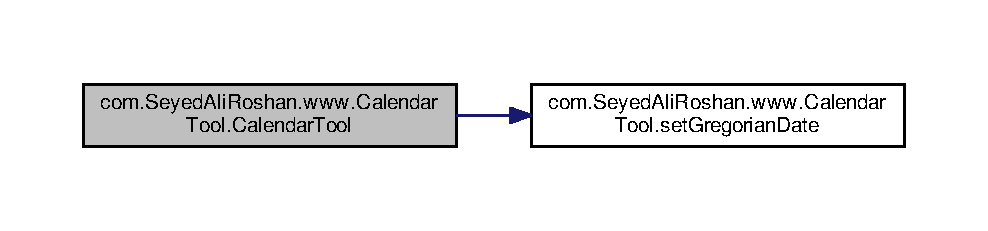
\includegraphics[width=350pt]{classcom_1_1_seyed_ali_roshan_1_1www_1_1_calendar_tool_a5bac292bba8e7a28dcdafe093072763a_cgraph}
\end{center}
\end{figure}


\index{com\+::\+Seyed\+Ali\+Roshan\+::www\+::\+Calendar\+Tool@{com\+::\+Seyed\+Ali\+Roshan\+::www\+::\+Calendar\+Tool}!Calendar\+Tool@{Calendar\+Tool}}
\index{Calendar\+Tool@{Calendar\+Tool}!com\+::\+Seyed\+Ali\+Roshan\+::www\+::\+Calendar\+Tool@{com\+::\+Seyed\+Ali\+Roshan\+::www\+::\+Calendar\+Tool}}
\subsubsection[{\texorpdfstring{Calendar\+Tool(int year, int month, int day)}{CalendarTool(int year, int month, int day)}}]{\setlength{\rightskip}{0pt plus 5cm}com.\+Seyed\+Ali\+Roshan.\+www.\+Calendar\+Tool.\+Calendar\+Tool (
\begin{DoxyParamCaption}
\item[{int}]{year, }
\item[{int}]{month, }
\item[{int}]{day}
\end{DoxyParamCaption}
)}\hypertarget{classcom_1_1_seyed_ali_roshan_1_1www_1_1_calendar_tool_a4cd03f8f1a3580a0a8d1fb56b535c028}{}\label{classcom_1_1_seyed_ali_roshan_1_1www_1_1_calendar_tool_a4cd03f8f1a3580a0a8d1fb56b535c028}
Java\+Source\+\_\+\+Calendar\+: This constructor receives a Gregorian date and initializes the other private members of the class accordingly.


\begin{DoxyParams}{Parameters}
{\em year} & int \\
\hline
{\em month} & int \\
\hline
{\em day} & int \\
\hline
\end{DoxyParams}


Definition at line 96 of file Calendar\+Tool.\+java.



Here is the call graph for this function\+:
\nopagebreak
\begin{figure}[H]
\begin{center}
\leavevmode
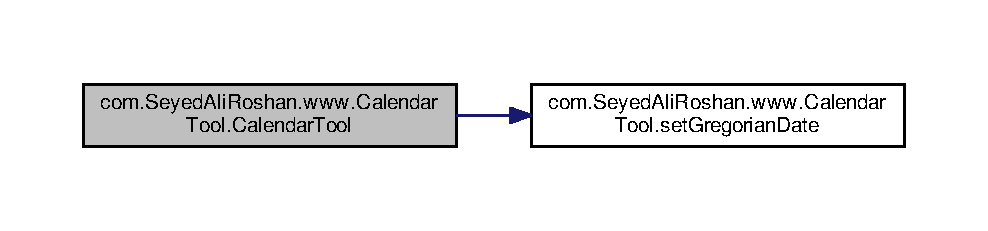
\includegraphics[width=350pt]{classcom_1_1_seyed_ali_roshan_1_1www_1_1_calendar_tool_a4cd03f8f1a3580a0a8d1fb56b535c028_cgraph}
\end{center}
\end{figure}




\subsection{Member Function Documentation}
\index{com\+::\+Seyed\+Ali\+Roshan\+::www\+::\+Calendar\+Tool@{com\+::\+Seyed\+Ali\+Roshan\+::www\+::\+Calendar\+Tool}!get\+Day\+Of\+Week@{get\+Day\+Of\+Week}}
\index{get\+Day\+Of\+Week@{get\+Day\+Of\+Week}!com\+::\+Seyed\+Ali\+Roshan\+::www\+::\+Calendar\+Tool@{com\+::\+Seyed\+Ali\+Roshan\+::www\+::\+Calendar\+Tool}}
\subsubsection[{\texorpdfstring{get\+Day\+Of\+Week()}{getDayOfWeek()}}]{\setlength{\rightskip}{0pt plus 5cm}int com.\+Seyed\+Ali\+Roshan.\+www.\+Calendar\+Tool.\+get\+Day\+Of\+Week (
\begin{DoxyParamCaption}
{}
\end{DoxyParamCaption}
)}\hypertarget{classcom_1_1_seyed_ali_roshan_1_1www_1_1_calendar_tool_a47c154df912d7c29f787e9724d5b19bf}{}\label{classcom_1_1_seyed_ali_roshan_1_1www_1_1_calendar_tool_a47c154df912d7c29f787e9724d5b19bf}
get\+Day\+Of\+Week\+: Returns the week day number. Monday=0..Sunday=6;

\begin{DoxyReturn}{Returns}
int 
\end{DoxyReturn}


Definition at line 297 of file Calendar\+Tool.\+java.



Here is the caller graph for this function\+:
\nopagebreak
\begin{figure}[H]
\begin{center}
\leavevmode
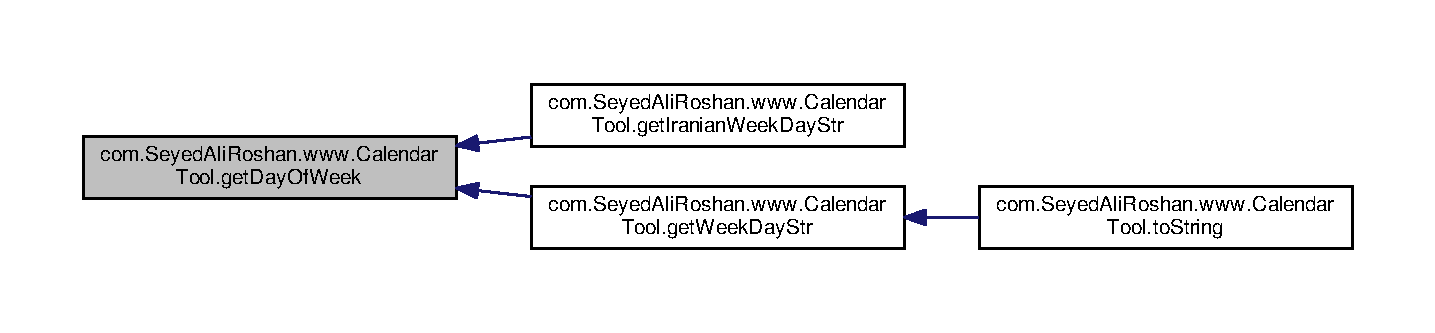
\includegraphics[width=350pt]{classcom_1_1_seyed_ali_roshan_1_1www_1_1_calendar_tool_a47c154df912d7c29f787e9724d5b19bf_icgraph}
\end{center}
\end{figure}


\index{com\+::\+Seyed\+Ali\+Roshan\+::www\+::\+Calendar\+Tool@{com\+::\+Seyed\+Ali\+Roshan\+::www\+::\+Calendar\+Tool}!get\+Gregorian\+Date@{get\+Gregorian\+Date}}
\index{get\+Gregorian\+Date@{get\+Gregorian\+Date}!com\+::\+Seyed\+Ali\+Roshan\+::www\+::\+Calendar\+Tool@{com\+::\+Seyed\+Ali\+Roshan\+::www\+::\+Calendar\+Tool}}
\subsubsection[{\texorpdfstring{get\+Gregorian\+Date()}{getGregorianDate()}}]{\setlength{\rightskip}{0pt plus 5cm}String com.\+Seyed\+Ali\+Roshan.\+www.\+Calendar\+Tool.\+get\+Gregorian\+Date (
\begin{DoxyParamCaption}
{}
\end{DoxyParamCaption}
)}\hypertarget{classcom_1_1_seyed_ali_roshan_1_1www_1_1_calendar_tool_a2d6513e1ec00cb12ee49728ec8879e20}{}\label{classcom_1_1_seyed_ali_roshan_1_1www_1_1_calendar_tool_a2d6513e1ec00cb12ee49728ec8879e20}
get\+Gregorian\+Date\+: Returns a string version of Gregorian date

\begin{DoxyReturn}{Returns}
String 
\end{DoxyReturn}


Definition at line 235 of file Calendar\+Tool.\+java.



Here is the caller graph for this function\+:
\nopagebreak
\begin{figure}[H]
\begin{center}
\leavevmode
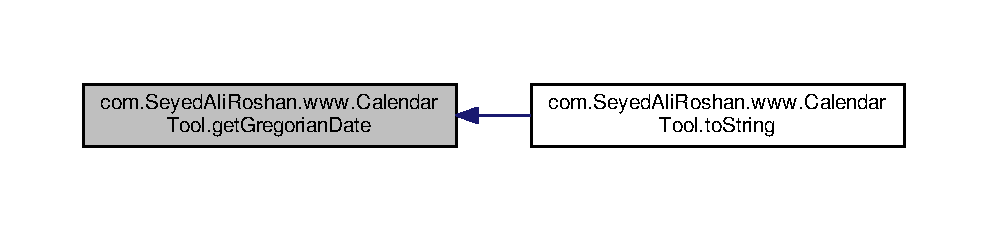
\includegraphics[width=350pt]{classcom_1_1_seyed_ali_roshan_1_1www_1_1_calendar_tool_a2d6513e1ec00cb12ee49728ec8879e20_icgraph}
\end{center}
\end{figure}


\index{com\+::\+Seyed\+Ali\+Roshan\+::www\+::\+Calendar\+Tool@{com\+::\+Seyed\+Ali\+Roshan\+::www\+::\+Calendar\+Tool}!get\+Gregorian\+Date@{get\+Gregorian\+Date}}
\index{get\+Gregorian\+Date@{get\+Gregorian\+Date}!com\+::\+Seyed\+Ali\+Roshan\+::www\+::\+Calendar\+Tool@{com\+::\+Seyed\+Ali\+Roshan\+::www\+::\+Calendar\+Tool}}
\subsubsection[{\texorpdfstring{get\+Gregorian\+Date(\+String Pattern)}{getGregorianDate(String Pattern)}}]{\setlength{\rightskip}{0pt plus 5cm}String com.\+Seyed\+Ali\+Roshan.\+www.\+Calendar\+Tool.\+get\+Gregorian\+Date (
\begin{DoxyParamCaption}
\item[{String}]{Pattern}
\end{DoxyParamCaption}
)}\hypertarget{classcom_1_1_seyed_ali_roshan_1_1www_1_1_calendar_tool_a64e054f39d6cf063e0abcb23c107761c}{}\label{classcom_1_1_seyed_ali_roshan_1_1www_1_1_calendar_tool_a64e054f39d6cf063e0abcb23c107761c}
get\+Gregorian\+Date\+: Returns a string version of Gregorian date which used user pattern as separator. \begin{DoxyAuthor}{Author}
Seyed Ali Roshan 
\end{DoxyAuthor}

\begin{DoxyParams}{Parameters}
{\em Pattern} & \\
\hline
\end{DoxyParams}
\begin{DoxyReturn}{Returns}
String 
\end{DoxyReturn}


Definition at line 246 of file Calendar\+Tool.\+java.

\index{com\+::\+Seyed\+Ali\+Roshan\+::www\+::\+Calendar\+Tool@{com\+::\+Seyed\+Ali\+Roshan\+::www\+::\+Calendar\+Tool}!get\+Gregorian\+Day@{get\+Gregorian\+Day}}
\index{get\+Gregorian\+Day@{get\+Gregorian\+Day}!com\+::\+Seyed\+Ali\+Roshan\+::www\+::\+Calendar\+Tool@{com\+::\+Seyed\+Ali\+Roshan\+::www\+::\+Calendar\+Tool}}
\subsubsection[{\texorpdfstring{get\+Gregorian\+Day()}{getGregorianDay()}}]{\setlength{\rightskip}{0pt plus 5cm}int com.\+Seyed\+Ali\+Roshan.\+www.\+Calendar\+Tool.\+get\+Gregorian\+Day (
\begin{DoxyParamCaption}
{}
\end{DoxyParamCaption}
)}\hypertarget{classcom_1_1_seyed_ali_roshan_1_1www_1_1_calendar_tool_a0f4bcde4f5df18120510c9db1d0bcd85}{}\label{classcom_1_1_seyed_ali_roshan_1_1www_1_1_calendar_tool_a0f4bcde4f5df18120510c9db1d0bcd85}
get\+Gregorian\+Day\+: Returns the \textquotesingle{}day\textquotesingle{} part of the Gregorian date.

\begin{DoxyReturn}{Returns}
int 
\end{DoxyReturn}


Definition at line 164 of file Calendar\+Tool.\+java.

\index{com\+::\+Seyed\+Ali\+Roshan\+::www\+::\+Calendar\+Tool@{com\+::\+Seyed\+Ali\+Roshan\+::www\+::\+Calendar\+Tool}!get\+Gregorian\+Month@{get\+Gregorian\+Month}}
\index{get\+Gregorian\+Month@{get\+Gregorian\+Month}!com\+::\+Seyed\+Ali\+Roshan\+::www\+::\+Calendar\+Tool@{com\+::\+Seyed\+Ali\+Roshan\+::www\+::\+Calendar\+Tool}}
\subsubsection[{\texorpdfstring{get\+Gregorian\+Month()}{getGregorianMonth()}}]{\setlength{\rightskip}{0pt plus 5cm}int com.\+Seyed\+Ali\+Roshan.\+www.\+Calendar\+Tool.\+get\+Gregorian\+Month (
\begin{DoxyParamCaption}
{}
\end{DoxyParamCaption}
)}\hypertarget{classcom_1_1_seyed_ali_roshan_1_1www_1_1_calendar_tool_a35f24d4098f8fdb9ce1134267679b007}{}\label{classcom_1_1_seyed_ali_roshan_1_1www_1_1_calendar_tool_a35f24d4098f8fdb9ce1134267679b007}
get\+Gregorian\+Month\+: Returns the \textquotesingle{}month\textquotesingle{} part of the Gregorian date.

\begin{DoxyReturn}{Returns}
int 
\end{DoxyReturn}


Definition at line 154 of file Calendar\+Tool.\+java.

\index{com\+::\+Seyed\+Ali\+Roshan\+::www\+::\+Calendar\+Tool@{com\+::\+Seyed\+Ali\+Roshan\+::www\+::\+Calendar\+Tool}!get\+Gregorian\+Year@{get\+Gregorian\+Year}}
\index{get\+Gregorian\+Year@{get\+Gregorian\+Year}!com\+::\+Seyed\+Ali\+Roshan\+::www\+::\+Calendar\+Tool@{com\+::\+Seyed\+Ali\+Roshan\+::www\+::\+Calendar\+Tool}}
\subsubsection[{\texorpdfstring{get\+Gregorian\+Year()}{getGregorianYear()}}]{\setlength{\rightskip}{0pt plus 5cm}int com.\+Seyed\+Ali\+Roshan.\+www.\+Calendar\+Tool.\+get\+Gregorian\+Year (
\begin{DoxyParamCaption}
{}
\end{DoxyParamCaption}
)}\hypertarget{classcom_1_1_seyed_ali_roshan_1_1www_1_1_calendar_tool_a75bd27aa8e56ff610fb24c5d8875f675}{}\label{classcom_1_1_seyed_ali_roshan_1_1www_1_1_calendar_tool_a75bd27aa8e56ff610fb24c5d8875f675}
get\+Gregorian\+Year\+: Returns the \textquotesingle{}year\textquotesingle{} part of the Gregorian date.

\begin{DoxyReturn}{Returns}
int 
\end{DoxyReturn}


Definition at line 144 of file Calendar\+Tool.\+java.

\index{com\+::\+Seyed\+Ali\+Roshan\+::www\+::\+Calendar\+Tool@{com\+::\+Seyed\+Ali\+Roshan\+::www\+::\+Calendar\+Tool}!get\+Iranian\+Date@{get\+Iranian\+Date}}
\index{get\+Iranian\+Date@{get\+Iranian\+Date}!com\+::\+Seyed\+Ali\+Roshan\+::www\+::\+Calendar\+Tool@{com\+::\+Seyed\+Ali\+Roshan\+::www\+::\+Calendar\+Tool}}
\subsubsection[{\texorpdfstring{get\+Iranian\+Date()}{getIranianDate()}}]{\setlength{\rightskip}{0pt plus 5cm}String com.\+Seyed\+Ali\+Roshan.\+www.\+Calendar\+Tool.\+get\+Iranian\+Date (
\begin{DoxyParamCaption}
{}
\end{DoxyParamCaption}
)}\hypertarget{classcom_1_1_seyed_ali_roshan_1_1www_1_1_calendar_tool_a77886e70247351f6f845fa88bdc8fa14}{}\label{classcom_1_1_seyed_ali_roshan_1_1www_1_1_calendar_tool_a77886e70247351f6f845fa88bdc8fa14}
get\+Iranian\+Date\+: Returns a string version of Iranian date

\begin{DoxyReturn}{Returns}
String 
\end{DoxyReturn}


Definition at line 204 of file Calendar\+Tool.\+java.



Here is the caller graph for this function\+:
\nopagebreak
\begin{figure}[H]
\begin{center}
\leavevmode
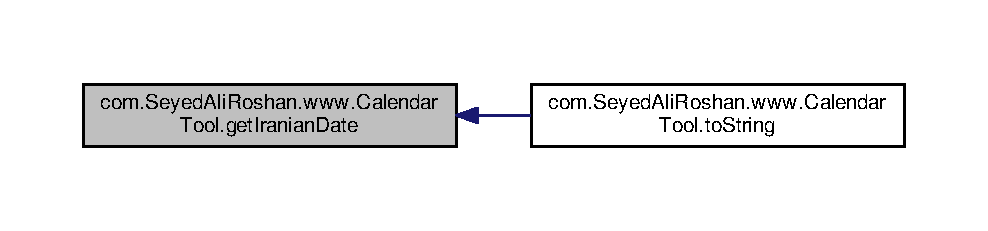
\includegraphics[width=350pt]{classcom_1_1_seyed_ali_roshan_1_1www_1_1_calendar_tool_a77886e70247351f6f845fa88bdc8fa14_icgraph}
\end{center}
\end{figure}


\index{com\+::\+Seyed\+Ali\+Roshan\+::www\+::\+Calendar\+Tool@{com\+::\+Seyed\+Ali\+Roshan\+::www\+::\+Calendar\+Tool}!get\+Iranian\+Date@{get\+Iranian\+Date}}
\index{get\+Iranian\+Date@{get\+Iranian\+Date}!com\+::\+Seyed\+Ali\+Roshan\+::www\+::\+Calendar\+Tool@{com\+::\+Seyed\+Ali\+Roshan\+::www\+::\+Calendar\+Tool}}
\subsubsection[{\texorpdfstring{get\+Iranian\+Date(\+String Pattern)}{getIranianDate(String Pattern)}}]{\setlength{\rightskip}{0pt plus 5cm}String com.\+Seyed\+Ali\+Roshan.\+www.\+Calendar\+Tool.\+get\+Iranian\+Date (
\begin{DoxyParamCaption}
\item[{String}]{Pattern}
\end{DoxyParamCaption}
)}\hypertarget{classcom_1_1_seyed_ali_roshan_1_1www_1_1_calendar_tool_af9a814c0d0be587f5598a479d35d6f7b}{}\label{classcom_1_1_seyed_ali_roshan_1_1www_1_1_calendar_tool_af9a814c0d0be587f5598a479d35d6f7b}
get\+Iranian\+Date\+: Returns a string version of Iranian date with user pattern separator. \begin{DoxyAuthor}{Author}
Seyed Ali Roshan 
\end{DoxyAuthor}

\begin{DoxyParams}{Parameters}
{\em Pattern} & \\
\hline
\end{DoxyParams}
\begin{DoxyReturn}{Returns}
String 
\end{DoxyReturn}


Definition at line 215 of file Calendar\+Tool.\+java.

\index{com\+::\+Seyed\+Ali\+Roshan\+::www\+::\+Calendar\+Tool@{com\+::\+Seyed\+Ali\+Roshan\+::www\+::\+Calendar\+Tool}!get\+Iranian\+Day@{get\+Iranian\+Day}}
\index{get\+Iranian\+Day@{get\+Iranian\+Day}!com\+::\+Seyed\+Ali\+Roshan\+::www\+::\+Calendar\+Tool@{com\+::\+Seyed\+Ali\+Roshan\+::www\+::\+Calendar\+Tool}}
\subsubsection[{\texorpdfstring{get\+Iranian\+Day()}{getIranianDay()}}]{\setlength{\rightskip}{0pt plus 5cm}int com.\+Seyed\+Ali\+Roshan.\+www.\+Calendar\+Tool.\+get\+Iranian\+Day (
\begin{DoxyParamCaption}
{}
\end{DoxyParamCaption}
)}\hypertarget{classcom_1_1_seyed_ali_roshan_1_1www_1_1_calendar_tool_adc0f3121df6416309d8837cfc2b3ef0c}{}\label{classcom_1_1_seyed_ali_roshan_1_1www_1_1_calendar_tool_adc0f3121df6416309d8837cfc2b3ef0c}
get\+Iranian\+Day\+: Returns the \textquotesingle{}day\textquotesingle{} part of the Iranian date.

\begin{DoxyReturn}{Returns}
int 
\end{DoxyReturn}


Definition at line 126 of file Calendar\+Tool.\+java.

\index{com\+::\+Seyed\+Ali\+Roshan\+::www\+::\+Calendar\+Tool@{com\+::\+Seyed\+Ali\+Roshan\+::www\+::\+Calendar\+Tool}!get\+Iranian\+Month@{get\+Iranian\+Month}}
\index{get\+Iranian\+Month@{get\+Iranian\+Month}!com\+::\+Seyed\+Ali\+Roshan\+::www\+::\+Calendar\+Tool@{com\+::\+Seyed\+Ali\+Roshan\+::www\+::\+Calendar\+Tool}}
\subsubsection[{\texorpdfstring{get\+Iranian\+Month()}{getIranianMonth()}}]{\setlength{\rightskip}{0pt plus 5cm}int com.\+Seyed\+Ali\+Roshan.\+www.\+Calendar\+Tool.\+get\+Iranian\+Month (
\begin{DoxyParamCaption}
{}
\end{DoxyParamCaption}
)}\hypertarget{classcom_1_1_seyed_ali_roshan_1_1www_1_1_calendar_tool_ae9011cd29c301785e51037c704bd6ee4}{}\label{classcom_1_1_seyed_ali_roshan_1_1www_1_1_calendar_tool_ae9011cd29c301785e51037c704bd6ee4}
get\+Iranian\+Month\+: Returns the \textquotesingle{}month\textquotesingle{} part of the Iranian date.

\begin{DoxyReturn}{Returns}
int 
\end{DoxyReturn}


Definition at line 116 of file Calendar\+Tool.\+java.



Here is the caller graph for this function\+:
\nopagebreak
\begin{figure}[H]
\begin{center}
\leavevmode
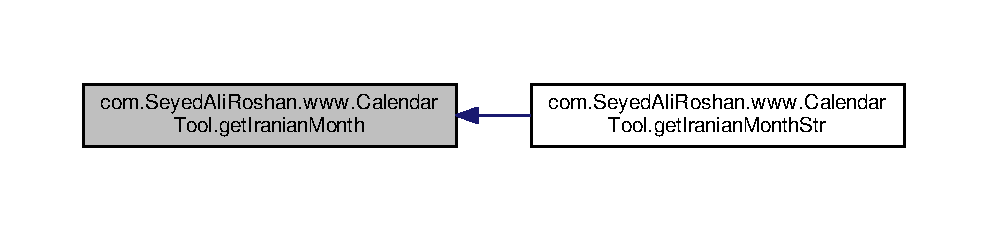
\includegraphics[width=350pt]{classcom_1_1_seyed_ali_roshan_1_1www_1_1_calendar_tool_ae9011cd29c301785e51037c704bd6ee4_icgraph}
\end{center}
\end{figure}


\index{com\+::\+Seyed\+Ali\+Roshan\+::www\+::\+Calendar\+Tool@{com\+::\+Seyed\+Ali\+Roshan\+::www\+::\+Calendar\+Tool}!get\+Iranian\+Month\+Str@{get\+Iranian\+Month\+Str}}
\index{get\+Iranian\+Month\+Str@{get\+Iranian\+Month\+Str}!com\+::\+Seyed\+Ali\+Roshan\+::www\+::\+Calendar\+Tool@{com\+::\+Seyed\+Ali\+Roshan\+::www\+::\+Calendar\+Tool}}
\subsubsection[{\texorpdfstring{get\+Iranian\+Month\+Str()}{getIranianMonthStr()}}]{\setlength{\rightskip}{0pt plus 5cm}String com.\+Seyed\+Ali\+Roshan.\+www.\+Calendar\+Tool.\+get\+Iranian\+Month\+Str (
\begin{DoxyParamCaption}
{}
\end{DoxyParamCaption}
)}\hypertarget{classcom_1_1_seyed_ali_roshan_1_1www_1_1_calendar_tool_a6f594c497638e8ab22b843429cd0c33c}{}\label{classcom_1_1_seyed_ali_roshan_1_1www_1_1_calendar_tool_a6f594c497638e8ab22b843429cd0c33c}


Definition at line 134 of file Calendar\+Tool.\+java.



Here is the call graph for this function\+:
\nopagebreak
\begin{figure}[H]
\begin{center}
\leavevmode
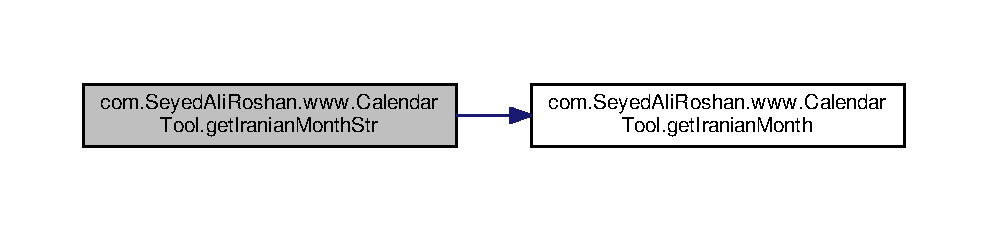
\includegraphics[width=350pt]{classcom_1_1_seyed_ali_roshan_1_1www_1_1_calendar_tool_a6f594c497638e8ab22b843429cd0c33c_cgraph}
\end{center}
\end{figure}


\index{com\+::\+Seyed\+Ali\+Roshan\+::www\+::\+Calendar\+Tool@{com\+::\+Seyed\+Ali\+Roshan\+::www\+::\+Calendar\+Tool}!get\+Iranian\+Week\+Day\+Str@{get\+Iranian\+Week\+Day\+Str}}
\index{get\+Iranian\+Week\+Day\+Str@{get\+Iranian\+Week\+Day\+Str}!com\+::\+Seyed\+Ali\+Roshan\+::www\+::\+Calendar\+Tool@{com\+::\+Seyed\+Ali\+Roshan\+::www\+::\+Calendar\+Tool}}
\subsubsection[{\texorpdfstring{get\+Iranian\+Week\+Day\+Str()}{getIranianWeekDayStr()}}]{\setlength{\rightskip}{0pt plus 5cm}String com.\+Seyed\+Ali\+Roshan.\+www.\+Calendar\+Tool.\+get\+Iranian\+Week\+Day\+Str (
\begin{DoxyParamCaption}
{}
\end{DoxyParamCaption}
)}\hypertarget{classcom_1_1_seyed_ali_roshan_1_1www_1_1_calendar_tool_a369f2b171ef0b5acfe4fb102033a87d4}{}\label{classcom_1_1_seyed_ali_roshan_1_1www_1_1_calendar_tool_a369f2b171ef0b5acfe4fb102033a87d4}


Definition at line 130 of file Calendar\+Tool.\+java.



Here is the call graph for this function\+:
\nopagebreak
\begin{figure}[H]
\begin{center}
\leavevmode
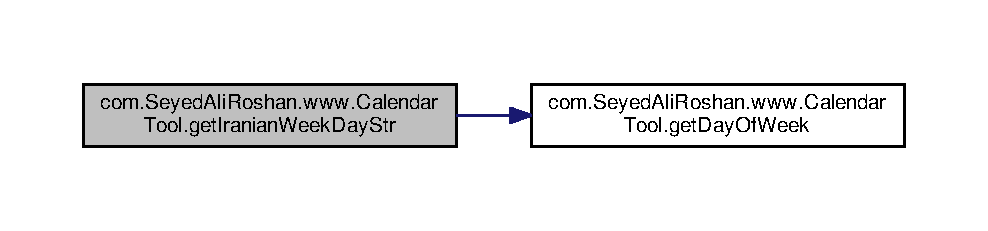
\includegraphics[width=350pt]{classcom_1_1_seyed_ali_roshan_1_1www_1_1_calendar_tool_a369f2b171ef0b5acfe4fb102033a87d4_cgraph}
\end{center}
\end{figure}


\index{com\+::\+Seyed\+Ali\+Roshan\+::www\+::\+Calendar\+Tool@{com\+::\+Seyed\+Ali\+Roshan\+::www\+::\+Calendar\+Tool}!get\+Iranian\+Year@{get\+Iranian\+Year}}
\index{get\+Iranian\+Year@{get\+Iranian\+Year}!com\+::\+Seyed\+Ali\+Roshan\+::www\+::\+Calendar\+Tool@{com\+::\+Seyed\+Ali\+Roshan\+::www\+::\+Calendar\+Tool}}
\subsubsection[{\texorpdfstring{get\+Iranian\+Year()}{getIranianYear()}}]{\setlength{\rightskip}{0pt plus 5cm}int com.\+Seyed\+Ali\+Roshan.\+www.\+Calendar\+Tool.\+get\+Iranian\+Year (
\begin{DoxyParamCaption}
{}
\end{DoxyParamCaption}
)}\hypertarget{classcom_1_1_seyed_ali_roshan_1_1www_1_1_calendar_tool_a032e77ba430be265ff9d55805237be5e}{}\label{classcom_1_1_seyed_ali_roshan_1_1www_1_1_calendar_tool_a032e77ba430be265ff9d55805237be5e}
get\+Iranian\+Year\+: Returns the \textquotesingle{}year\textquotesingle{} part of the Iranian date.

\begin{DoxyReturn}{Returns}
int 
\end{DoxyReturn}


Definition at line 106 of file Calendar\+Tool.\+java.

\index{com\+::\+Seyed\+Ali\+Roshan\+::www\+::\+Calendar\+Tool@{com\+::\+Seyed\+Ali\+Roshan\+::www\+::\+Calendar\+Tool}!get\+Julian\+Date@{get\+Julian\+Date}}
\index{get\+Julian\+Date@{get\+Julian\+Date}!com\+::\+Seyed\+Ali\+Roshan\+::www\+::\+Calendar\+Tool@{com\+::\+Seyed\+Ali\+Roshan\+::www\+::\+Calendar\+Tool}}
\subsubsection[{\texorpdfstring{get\+Julian\+Date()}{getJulianDate()}}]{\setlength{\rightskip}{0pt plus 5cm}String com.\+Seyed\+Ali\+Roshan.\+www.\+Calendar\+Tool.\+get\+Julian\+Date (
\begin{DoxyParamCaption}
{}
\end{DoxyParamCaption}
)}\hypertarget{classcom_1_1_seyed_ali_roshan_1_1www_1_1_calendar_tool_ae0c8c9034e150da4d8442f374244cab3}{}\label{classcom_1_1_seyed_ali_roshan_1_1www_1_1_calendar_tool_ae0c8c9034e150da4d8442f374244cab3}
get\+Julian\+Date\+: Returns a string version of Julian date

\begin{DoxyReturn}{Returns}
String 
\end{DoxyReturn}


Definition at line 256 of file Calendar\+Tool.\+java.



Here is the caller graph for this function\+:
\nopagebreak
\begin{figure}[H]
\begin{center}
\leavevmode
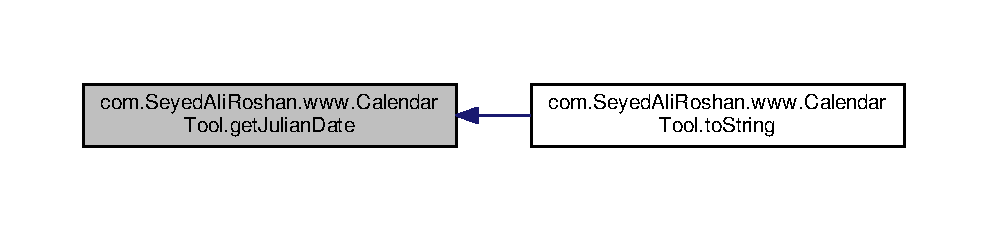
\includegraphics[width=350pt]{classcom_1_1_seyed_ali_roshan_1_1www_1_1_calendar_tool_ae0c8c9034e150da4d8442f374244cab3_icgraph}
\end{center}
\end{figure}


\index{com\+::\+Seyed\+Ali\+Roshan\+::www\+::\+Calendar\+Tool@{com\+::\+Seyed\+Ali\+Roshan\+::www\+::\+Calendar\+Tool}!get\+Julian\+Day@{get\+Julian\+Day}}
\index{get\+Julian\+Day@{get\+Julian\+Day}!com\+::\+Seyed\+Ali\+Roshan\+::www\+::\+Calendar\+Tool@{com\+::\+Seyed\+Ali\+Roshan\+::www\+::\+Calendar\+Tool}}
\subsubsection[{\texorpdfstring{get\+Julian\+Day()}{getJulianDay()}}]{\setlength{\rightskip}{0pt plus 5cm}int com.\+Seyed\+Ali\+Roshan.\+www.\+Calendar\+Tool.\+get\+Julian\+Day (
\begin{DoxyParamCaption}
{}
\end{DoxyParamCaption}
)}\hypertarget{classcom_1_1_seyed_ali_roshan_1_1www_1_1_calendar_tool_a41147d1ef316a32e2db40eed38022496}{}\label{classcom_1_1_seyed_ali_roshan_1_1www_1_1_calendar_tool_a41147d1ef316a32e2db40eed38022496}
\hyperlink{classcom_1_1_seyed_ali_roshan_1_1www_1_1_calendar_tool_a41147d1ef316a32e2db40eed38022496}{get\+Julian\+Day()} Returns the \textquotesingle{}day\textquotesingle{} part of the Julian date.

\begin{DoxyReturn}{Returns}
int 
\end{DoxyReturn}


Definition at line 194 of file Calendar\+Tool.\+java.

\index{com\+::\+Seyed\+Ali\+Roshan\+::www\+::\+Calendar\+Tool@{com\+::\+Seyed\+Ali\+Roshan\+::www\+::\+Calendar\+Tool}!get\+Julian\+Month@{get\+Julian\+Month}}
\index{get\+Julian\+Month@{get\+Julian\+Month}!com\+::\+Seyed\+Ali\+Roshan\+::www\+::\+Calendar\+Tool@{com\+::\+Seyed\+Ali\+Roshan\+::www\+::\+Calendar\+Tool}}
\subsubsection[{\texorpdfstring{get\+Julian\+Month()}{getJulianMonth()}}]{\setlength{\rightskip}{0pt plus 5cm}int com.\+Seyed\+Ali\+Roshan.\+www.\+Calendar\+Tool.\+get\+Julian\+Month (
\begin{DoxyParamCaption}
{}
\end{DoxyParamCaption}
)}\hypertarget{classcom_1_1_seyed_ali_roshan_1_1www_1_1_calendar_tool_a55ec1b9e58157723f2ea6a5d4167a3f0}{}\label{classcom_1_1_seyed_ali_roshan_1_1www_1_1_calendar_tool_a55ec1b9e58157723f2ea6a5d4167a3f0}
get\+Julian\+Month\+: Returns the \textquotesingle{}month\textquotesingle{} part of the Julian date.

\begin{DoxyReturn}{Returns}
int 
\end{DoxyReturn}


Definition at line 184 of file Calendar\+Tool.\+java.

\index{com\+::\+Seyed\+Ali\+Roshan\+::www\+::\+Calendar\+Tool@{com\+::\+Seyed\+Ali\+Roshan\+::www\+::\+Calendar\+Tool}!get\+Julian\+Year@{get\+Julian\+Year}}
\index{get\+Julian\+Year@{get\+Julian\+Year}!com\+::\+Seyed\+Ali\+Roshan\+::www\+::\+Calendar\+Tool@{com\+::\+Seyed\+Ali\+Roshan\+::www\+::\+Calendar\+Tool}}
\subsubsection[{\texorpdfstring{get\+Julian\+Year()}{getJulianYear()}}]{\setlength{\rightskip}{0pt plus 5cm}int com.\+Seyed\+Ali\+Roshan.\+www.\+Calendar\+Tool.\+get\+Julian\+Year (
\begin{DoxyParamCaption}
{}
\end{DoxyParamCaption}
)}\hypertarget{classcom_1_1_seyed_ali_roshan_1_1www_1_1_calendar_tool_a61e6dae7e20420b13cd99871d3ec83cd}{}\label{classcom_1_1_seyed_ali_roshan_1_1www_1_1_calendar_tool_a61e6dae7e20420b13cd99871d3ec83cd}
get\+Julian\+Year\+: Returns the \textquotesingle{}year\textquotesingle{} part of the Julian date.

\begin{DoxyReturn}{Returns}
int 
\end{DoxyReturn}


Definition at line 174 of file Calendar\+Tool.\+java.

\index{com\+::\+Seyed\+Ali\+Roshan\+::www\+::\+Calendar\+Tool@{com\+::\+Seyed\+Ali\+Roshan\+::www\+::\+Calendar\+Tool}!get\+Week\+Day\+Str@{get\+Week\+Day\+Str}}
\index{get\+Week\+Day\+Str@{get\+Week\+Day\+Str}!com\+::\+Seyed\+Ali\+Roshan\+::www\+::\+Calendar\+Tool@{com\+::\+Seyed\+Ali\+Roshan\+::www\+::\+Calendar\+Tool}}
\subsubsection[{\texorpdfstring{get\+Week\+Day\+Str()}{getWeekDayStr()}}]{\setlength{\rightskip}{0pt plus 5cm}String com.\+Seyed\+Ali\+Roshan.\+www.\+Calendar\+Tool.\+get\+Week\+Day\+Str (
\begin{DoxyParamCaption}
{}
\end{DoxyParamCaption}
)}\hypertarget{classcom_1_1_seyed_ali_roshan_1_1www_1_1_calendar_tool_a04489ed109d9d4d88b12ef7cfe6d84c8}{}\label{classcom_1_1_seyed_ali_roshan_1_1www_1_1_calendar_tool_a04489ed109d9d4d88b12ef7cfe6d84c8}
get\+Week\+Day\+Str\+: Returns the week day name.

\begin{DoxyReturn}{Returns}
String 
\end{DoxyReturn}


Definition at line 266 of file Calendar\+Tool.\+java.



Here is the call graph for this function\+:
\nopagebreak
\begin{figure}[H]
\begin{center}
\leavevmode
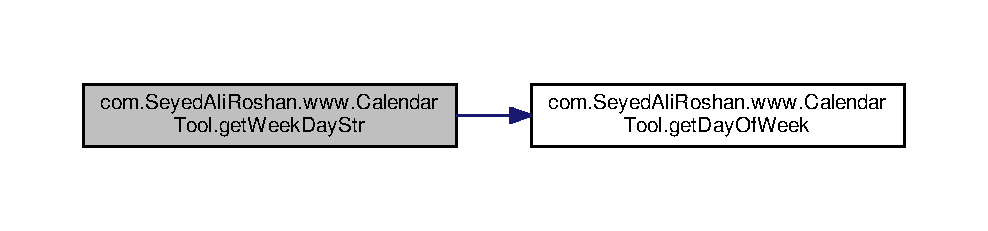
\includegraphics[width=350pt]{classcom_1_1_seyed_ali_roshan_1_1www_1_1_calendar_tool_a04489ed109d9d4d88b12ef7cfe6d84c8_cgraph}
\end{center}
\end{figure}




Here is the caller graph for this function\+:
\nopagebreak
\begin{figure}[H]
\begin{center}
\leavevmode
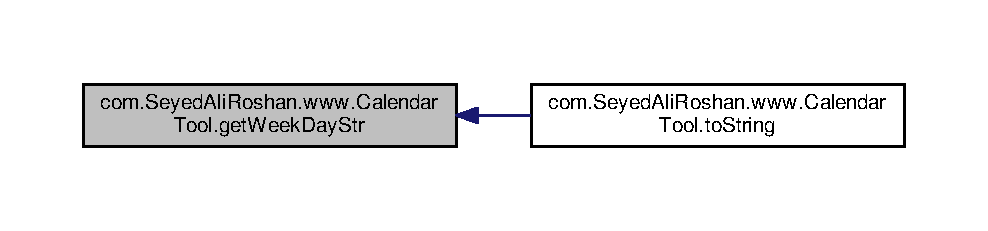
\includegraphics[width=350pt]{classcom_1_1_seyed_ali_roshan_1_1www_1_1_calendar_tool_a04489ed109d9d4d88b12ef7cfe6d84c8_icgraph}
\end{center}
\end{figure}


\index{com\+::\+Seyed\+Ali\+Roshan\+::www\+::\+Calendar\+Tool@{com\+::\+Seyed\+Ali\+Roshan\+::www\+::\+Calendar\+Tool}!Is\+Leap@{Is\+Leap}}
\index{Is\+Leap@{Is\+Leap}!com\+::\+Seyed\+Ali\+Roshan\+::www\+::\+Calendar\+Tool@{com\+::\+Seyed\+Ali\+Roshan\+::www\+::\+Calendar\+Tool}}
\subsubsection[{\texorpdfstring{Is\+Leap(int ir\+Year1)}{IsLeap(int irYear1)}}]{\setlength{\rightskip}{0pt plus 5cm}boolean com.\+Seyed\+Ali\+Roshan.\+www.\+Calendar\+Tool.\+Is\+Leap (
\begin{DoxyParamCaption}
\item[{int}]{ir\+Year1}
\end{DoxyParamCaption}
)}\hypertarget{classcom_1_1_seyed_ali_roshan_1_1www_1_1_calendar_tool_a281b3d746597ab1d1c5b0509407017b6}{}\label{classcom_1_1_seyed_ali_roshan_1_1www_1_1_calendar_tool_a281b3d746597ab1d1c5b0509407017b6}
Is\+Leap\+: This method determines if the Iranian (Jalali) year is leap (366-\/day long) or is the common year (365 days), and finds the day in March (Gregorian Calendar)of the first day of the Iranian year (\textquotesingle{}ir\+Year\textquotesingle{}).Iranian year (ir\+Year) ranges from (-\/61 to 3177).This method will set the following private data members as follows\+: leap\+: Number of years since the last leap year (0 to 4) Gy\+: Gregorian year of the begining of Iranian year march\+: The March day of Farvardin the 1st (first day of ja\+Year) 

Definition at line 464 of file Calendar\+Tool.\+java.

\index{com\+::\+Seyed\+Ali\+Roshan\+::www\+::\+Calendar\+Tool@{com\+::\+Seyed\+Ali\+Roshan\+::www\+::\+Calendar\+Tool}!next\+Day@{next\+Day}}
\index{next\+Day@{next\+Day}!com\+::\+Seyed\+Ali\+Roshan\+::www\+::\+Calendar\+Tool@{com\+::\+Seyed\+Ali\+Roshan\+::www\+::\+Calendar\+Tool}}
\subsubsection[{\texorpdfstring{next\+Day()}{nextDay()}}]{\setlength{\rightskip}{0pt plus 5cm}void com.\+Seyed\+Ali\+Roshan.\+www.\+Calendar\+Tool.\+next\+Day (
\begin{DoxyParamCaption}
{}
\end{DoxyParamCaption}
)}\hypertarget{classcom_1_1_seyed_ali_roshan_1_1www_1_1_calendar_tool_ab59e8a3ee76803057ef8210f6d7a9bbd}{}\label{classcom_1_1_seyed_ali_roshan_1_1www_1_1_calendar_tool_ab59e8a3ee76803057ef8210f6d7a9bbd}
next\+Day\+: Go to next julian day number (J\+DN) and adjusts the other dates. 

Definition at line 305 of file Calendar\+Tool.\+java.

\index{com\+::\+Seyed\+Ali\+Roshan\+::www\+::\+Calendar\+Tool@{com\+::\+Seyed\+Ali\+Roshan\+::www\+::\+Calendar\+Tool}!next\+Day@{next\+Day}}
\index{next\+Day@{next\+Day}!com\+::\+Seyed\+Ali\+Roshan\+::www\+::\+Calendar\+Tool@{com\+::\+Seyed\+Ali\+Roshan\+::www\+::\+Calendar\+Tool}}
\subsubsection[{\texorpdfstring{next\+Day(int days)}{nextDay(int days)}}]{\setlength{\rightskip}{0pt plus 5cm}void com.\+Seyed\+Ali\+Roshan.\+www.\+Calendar\+Tool.\+next\+Day (
\begin{DoxyParamCaption}
\item[{int}]{days}
\end{DoxyParamCaption}
)}\hypertarget{classcom_1_1_seyed_ali_roshan_1_1www_1_1_calendar_tool_a52daf9e8935afad5dff3e1482c47bc30}{}\label{classcom_1_1_seyed_ali_roshan_1_1www_1_1_calendar_tool_a52daf9e8935afad5dff3e1482c47bc30}
next\+Day\+: Overload the \hyperlink{classcom_1_1_seyed_ali_roshan_1_1www_1_1_calendar_tool_ab59e8a3ee76803057ef8210f6d7a9bbd}{next\+Day()} method to accept the number of days to go ahead and adjusts the other dates accordingly.


\begin{DoxyParams}{Parameters}
{\em days} & int \\
\hline
\end{DoxyParams}


Definition at line 319 of file Calendar\+Tool.\+java.

\index{com\+::\+Seyed\+Ali\+Roshan\+::www\+::\+Calendar\+Tool@{com\+::\+Seyed\+Ali\+Roshan\+::www\+::\+Calendar\+Tool}!previous\+Day@{previous\+Day}}
\index{previous\+Day@{previous\+Day}!com\+::\+Seyed\+Ali\+Roshan\+::www\+::\+Calendar\+Tool@{com\+::\+Seyed\+Ali\+Roshan\+::www\+::\+Calendar\+Tool}}
\subsubsection[{\texorpdfstring{previous\+Day()}{previousDay()}}]{\setlength{\rightskip}{0pt plus 5cm}void com.\+Seyed\+Ali\+Roshan.\+www.\+Calendar\+Tool.\+previous\+Day (
\begin{DoxyParamCaption}
{}
\end{DoxyParamCaption}
)}\hypertarget{classcom_1_1_seyed_ali_roshan_1_1www_1_1_calendar_tool_aba478ff987023dc1b76c9e58193a59f4}{}\label{classcom_1_1_seyed_ali_roshan_1_1www_1_1_calendar_tool_aba478ff987023dc1b76c9e58193a59f4}
previous\+Day\+: Go to previous julian day number (J\+DN) and adjusts the otehr dates. 

Definition at line 330 of file Calendar\+Tool.\+java.

\index{com\+::\+Seyed\+Ali\+Roshan\+::www\+::\+Calendar\+Tool@{com\+::\+Seyed\+Ali\+Roshan\+::www\+::\+Calendar\+Tool}!previous\+Day@{previous\+Day}}
\index{previous\+Day@{previous\+Day}!com\+::\+Seyed\+Ali\+Roshan\+::www\+::\+Calendar\+Tool@{com\+::\+Seyed\+Ali\+Roshan\+::www\+::\+Calendar\+Tool}}
\subsubsection[{\texorpdfstring{previous\+Day(int days)}{previousDay(int days)}}]{\setlength{\rightskip}{0pt plus 5cm}void com.\+Seyed\+Ali\+Roshan.\+www.\+Calendar\+Tool.\+previous\+Day (
\begin{DoxyParamCaption}
\item[{int}]{days}
\end{DoxyParamCaption}
)}\hypertarget{classcom_1_1_seyed_ali_roshan_1_1www_1_1_calendar_tool_a00d787ebbcd21fb884e0e6708b88fe84}{}\label{classcom_1_1_seyed_ali_roshan_1_1www_1_1_calendar_tool_a00d787ebbcd21fb884e0e6708b88fe84}
previous\+Day\+: Overload the \hyperlink{classcom_1_1_seyed_ali_roshan_1_1www_1_1_calendar_tool_aba478ff987023dc1b76c9e58193a59f4}{previous\+Day()} method to accept the number of days to go backward and adjusts the other dates accordingly.


\begin{DoxyParams}{Parameters}
{\em days} & int \\
\hline
\end{DoxyParams}


Definition at line 344 of file Calendar\+Tool.\+java.

\index{com\+::\+Seyed\+Ali\+Roshan\+::www\+::\+Calendar\+Tool@{com\+::\+Seyed\+Ali\+Roshan\+::www\+::\+Calendar\+Tool}!set\+Gregorian\+Date@{set\+Gregorian\+Date}}
\index{set\+Gregorian\+Date@{set\+Gregorian\+Date}!com\+::\+Seyed\+Ali\+Roshan\+::www\+::\+Calendar\+Tool@{com\+::\+Seyed\+Ali\+Roshan\+::www\+::\+Calendar\+Tool}}
\subsubsection[{\texorpdfstring{set\+Gregorian\+Date(int year, int month, int day)}{setGregorianDate(int year, int month, int day)}}]{\setlength{\rightskip}{0pt plus 5cm}void com.\+Seyed\+Ali\+Roshan.\+www.\+Calendar\+Tool.\+set\+Gregorian\+Date (
\begin{DoxyParamCaption}
\item[{int}]{year, }
\item[{int}]{month, }
\item[{int}]{day}
\end{DoxyParamCaption}
)}\hypertarget{classcom_1_1_seyed_ali_roshan_1_1www_1_1_calendar_tool_a6299181390578255631f827c7bb1f358}{}\label{classcom_1_1_seyed_ali_roshan_1_1www_1_1_calendar_tool_a6299181390578255631f827c7bb1f358}
set\+Gregorian\+Date\+: Sets the date according to the Gregorian calendar and adjusts the other dates.


\begin{DoxyParams}{Parameters}
{\em year} & int \\
\hline
{\em month} & int \\
\hline
{\em day} & int \\
\hline
\end{DoxyParams}


Definition at line 377 of file Calendar\+Tool.\+java.



Here is the caller graph for this function\+:
\nopagebreak
\begin{figure}[H]
\begin{center}
\leavevmode
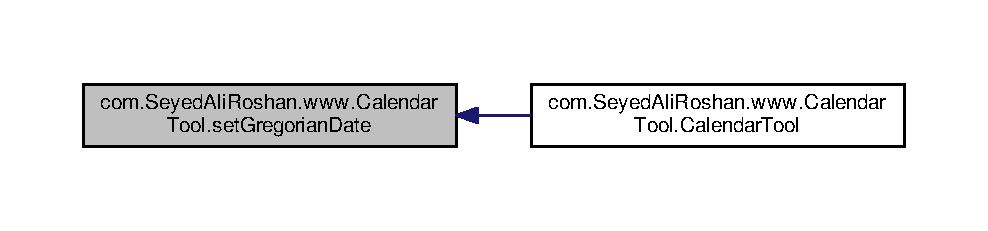
\includegraphics[width=350pt]{classcom_1_1_seyed_ali_roshan_1_1www_1_1_calendar_tool_a6299181390578255631f827c7bb1f358_icgraph}
\end{center}
\end{figure}


\index{com\+::\+Seyed\+Ali\+Roshan\+::www\+::\+Calendar\+Tool@{com\+::\+Seyed\+Ali\+Roshan\+::www\+::\+Calendar\+Tool}!set\+Iranian\+Date@{set\+Iranian\+Date}}
\index{set\+Iranian\+Date@{set\+Iranian\+Date}!com\+::\+Seyed\+Ali\+Roshan\+::www\+::\+Calendar\+Tool@{com\+::\+Seyed\+Ali\+Roshan\+::www\+::\+Calendar\+Tool}}
\subsubsection[{\texorpdfstring{set\+Iranian\+Date(\+String jalali\+Air\+Date)}{setIranianDate(String jalaliAirDate)}}]{\setlength{\rightskip}{0pt plus 5cm}void com.\+Seyed\+Ali\+Roshan.\+www.\+Calendar\+Tool.\+set\+Iranian\+Date (
\begin{DoxyParamCaption}
\item[{String}]{jalali\+Air\+Date}
\end{DoxyParamCaption}
)}\hypertarget{classcom_1_1_seyed_ali_roshan_1_1www_1_1_calendar_tool_a9995342b318abf5e7ef064432501f06a}{}\label{classcom_1_1_seyed_ali_roshan_1_1www_1_1_calendar_tool_a9995342b318abf5e7ef064432501f06a}


Definition at line 219 of file Calendar\+Tool.\+java.

\index{com\+::\+Seyed\+Ali\+Roshan\+::www\+::\+Calendar\+Tool@{com\+::\+Seyed\+Ali\+Roshan\+::www\+::\+Calendar\+Tool}!set\+Iranian\+Date@{set\+Iranian\+Date}}
\index{set\+Iranian\+Date@{set\+Iranian\+Date}!com\+::\+Seyed\+Ali\+Roshan\+::www\+::\+Calendar\+Tool@{com\+::\+Seyed\+Ali\+Roshan\+::www\+::\+Calendar\+Tool}}
\subsubsection[{\texorpdfstring{set\+Iranian\+Date(int year, int month, int day)}{setIranianDate(int year, int month, int day)}}]{\setlength{\rightskip}{0pt plus 5cm}void com.\+Seyed\+Ali\+Roshan.\+www.\+Calendar\+Tool.\+set\+Iranian\+Date (
\begin{DoxyParamCaption}
\item[{int}]{year, }
\item[{int}]{month, }
\item[{int}]{day}
\end{DoxyParamCaption}
)}\hypertarget{classcom_1_1_seyed_ali_roshan_1_1www_1_1_calendar_tool_abc55d566a57a157009a5c40b7a0fb53f}{}\label{classcom_1_1_seyed_ali_roshan_1_1www_1_1_calendar_tool_abc55d566a57a157009a5c40b7a0fb53f}
set\+Iranian\+Date\+: Sets the date according to the Iranian calendar and adjusts the other dates.


\begin{DoxyParams}{Parameters}
{\em year} & int \\
\hline
{\em month} & int \\
\hline
{\em day} & int \\
\hline
\end{DoxyParams}


Definition at line 359 of file Calendar\+Tool.\+java.

\index{com\+::\+Seyed\+Ali\+Roshan\+::www\+::\+Calendar\+Tool@{com\+::\+Seyed\+Ali\+Roshan\+::www\+::\+Calendar\+Tool}!set\+Julian\+Date@{set\+Julian\+Date}}
\index{set\+Julian\+Date@{set\+Julian\+Date}!com\+::\+Seyed\+Ali\+Roshan\+::www\+::\+Calendar\+Tool@{com\+::\+Seyed\+Ali\+Roshan\+::www\+::\+Calendar\+Tool}}
\subsubsection[{\texorpdfstring{set\+Julian\+Date(int year, int month, int day)}{setJulianDate(int year, int month, int day)}}]{\setlength{\rightskip}{0pt plus 5cm}void com.\+Seyed\+Ali\+Roshan.\+www.\+Calendar\+Tool.\+set\+Julian\+Date (
\begin{DoxyParamCaption}
\item[{int}]{year, }
\item[{int}]{month, }
\item[{int}]{day}
\end{DoxyParamCaption}
)}\hypertarget{classcom_1_1_seyed_ali_roshan_1_1www_1_1_calendar_tool_ae50de6d166135c2b5b7d107d37ca201e}{}\label{classcom_1_1_seyed_ali_roshan_1_1www_1_1_calendar_tool_ae50de6d166135c2b5b7d107d37ca201e}
set\+Julian\+Date\+: Sets the date according to the Julian calendar and adjusts the other dates.


\begin{DoxyParams}{Parameters}
{\em year} & int \\
\hline
{\em month} & int \\
\hline
{\em day} & int \\
\hline
\end{DoxyParams}


Definition at line 395 of file Calendar\+Tool.\+java.

\index{com\+::\+Seyed\+Ali\+Roshan\+::www\+::\+Calendar\+Tool@{com\+::\+Seyed\+Ali\+Roshan\+::www\+::\+Calendar\+Tool}!to\+String@{to\+String}}
\index{to\+String@{to\+String}!com\+::\+Seyed\+Ali\+Roshan\+::www\+::\+Calendar\+Tool@{com\+::\+Seyed\+Ali\+Roshan\+::www\+::\+Calendar\+Tool}}
\subsubsection[{\texorpdfstring{to\+String()}{toString()}}]{\setlength{\rightskip}{0pt plus 5cm}String com.\+Seyed\+Ali\+Roshan.\+www.\+Calendar\+Tool.\+to\+String (
\begin{DoxyParamCaption}
{}
\end{DoxyParamCaption}
)}\hypertarget{classcom_1_1_seyed_ali_roshan_1_1www_1_1_calendar_tool_ad236b0b986cfd9a5d4c62c1fd2b3e836}{}\label{classcom_1_1_seyed_ali_roshan_1_1www_1_1_calendar_tool_ad236b0b986cfd9a5d4c62c1fd2b3e836}
to\+String\+: Overrides the default \hyperlink{classcom_1_1_seyed_ali_roshan_1_1www_1_1_calendar_tool_ad236b0b986cfd9a5d4c62c1fd2b3e836}{to\+String()} method to return all dates.

\begin{DoxyReturn}{Returns}
String 
\end{DoxyReturn}


Definition at line 284 of file Calendar\+Tool.\+java.



Here is the call graph for this function\+:
\nopagebreak
\begin{figure}[H]
\begin{center}
\leavevmode
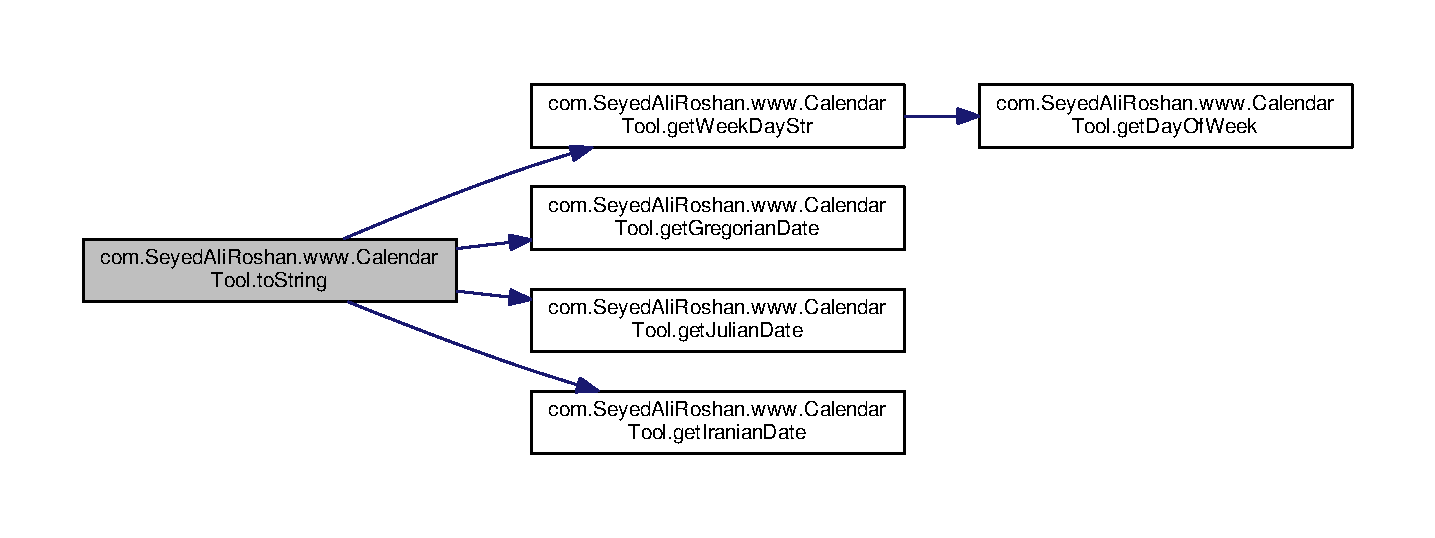
\includegraphics[width=350pt]{classcom_1_1_seyed_ali_roshan_1_1www_1_1_calendar_tool_ad236b0b986cfd9a5d4c62c1fd2b3e836_cgraph}
\end{center}
\end{figure}




The documentation for this class was generated from the following file\+:\begin{DoxyCompactItemize}
\item 
/home/seyed/\+Net\+Beans\+Projects/\+Calendar\+Parser/src/com/\+Seyed\+Ali\+Roshan/www/\hyperlink{_calendar_tool_8java}{Calendar\+Tool.\+java}\end{DoxyCompactItemize}

\chapter{File Documentation}
\hypertarget{_calendar_tool_8java}{}\section{/home/seyed/\+Net\+Beans\+Projects/\+Calendar\+Parser/src/com/\+Seyed\+Ali\+Roshan/www/\+Calendar\+Tool.java File Reference}
\label{_calendar_tool_8java}\index{/home/seyed/\+Net\+Beans\+Projects/\+Calendar\+Parser/src/com/\+Seyed\+Ali\+Roshan/www/\+Calendar\+Tool.\+java@{/home/seyed/\+Net\+Beans\+Projects/\+Calendar\+Parser/src/com/\+Seyed\+Ali\+Roshan/www/\+Calendar\+Tool.\+java}}
\subsection*{Classes}
\begin{DoxyCompactItemize}
\item 
class \hyperlink{classcom_1_1_seyed_ali_roshan_1_1www_1_1_calendar_tool}{com.\+Seyed\+Ali\+Roshan.\+www.\+Calendar\+Tool}
\end{DoxyCompactItemize}
\subsection*{Packages}
\begin{DoxyCompactItemize}
\item 
package \hyperlink{namespacecom_1_1_seyed_ali_roshan_1_1www}{com.\+Seyed\+Ali\+Roshan.\+www}
\end{DoxyCompactItemize}

%--- End generated contents ---

% Index
\backmatter
\newpage
\phantomsection
\clearemptydoublepage
\addcontentsline{toc}{chapter}{Index}
\printindex

\end{document}
